\section{Процессы переноса в газах}

\noindent
\textbf{Длина свободного пробега, время свободного пробега:}
\begin{equation}
    l = \frac{1}{n \sigma}, \hspace{1cm} \tau = \frac{1}{n \overline{v} \sigma}
\end{equation}

\noindent
\textbf{Закон Фурье:}
\begin{equation}
    \boxed{\vc{q} = - \varkappa \nabla(T) }
\end{equation}

\noindent
\textbf{Сила вязкого трения (закон Ньютона):} 
\begin{equation}
    \boxed{F_x/S = - \eta \frac{du_x}{dy}}
\end{equation}

\noindent
\textbf{Коэффициент\footnote{
    $l \sim 1/(n \sigma)$, $n \sim P/T$, $\overline{v} \sim \sqrt{T/m}$
} диффузии:}
\begin{equation}
    j = \frac{N^{\uparrow} - N^{\downarrow}}{\tau} \approx - \frac{1}{3} \overline{v} l \frac{dn}{dx} \Rightarrow D = \frac{1}{3}\overline{v}l, \;\; \text{или } D \sim \frac{T^{3/2}}{P \sqrt{m}} 
\end{equation}

\noindent
\textbf{Коэффициент теплопроводности:}

\begin{equation}
    \varkappa = \frac{1}{3}\overline{v} l n c_V = C_V D
\end{equation}

\begin{proof}[$\triangle$]
Рассмотрим тепловой поток:
$$
q = \frac{\varepsilon(x-l) N^{\uparrow} - \varepsilon (x + l) N^{\downarrow}}{\tau} = - N^{\uparrow} \frac{2l}{\tau} \frac{d \varepsilon(x)}{dx} = - \frac{1}{3} n \overline{v} l c_V \frac{dT}{dx}
$$
\end{proof}

\noindent
\textbf{Коэффициент вязкости:}
\begin{equation}
    \eta = \frac{1}{3} \rho \overline{v} l = \rho D
\end{equation}

\begin{proof}[$\triangle$]
\com{
Вязкость -- перенос тангнциальной компоненты импульса в гарравлении, перпендикулярном скорости течения.
Тогда
$$p_z^{\uparrow} = mu (x-l) N^{\uparrow}, 
p_z^{\downarrow} = mu (x+l) N^{\downarrow}$$
Тогда сила трения на верхний слой со стороны нижнего (на единицу площади) равна
$$
\digamma_z = \frac{\Delta p_z}{\tau} = - N^{\uparrow} \frac{2lm}{\tau} \frac{du(x)}{dx} = -\frac{1}{3} m n \overline{v} l \frac{du}{dx}
$$}
\end{proof}

\noindent
\textbf{Формула\footnote{
    Из ЗСИ и ЗСЭ.
} Сазерленда}
\begin{equation}
    \sigma = \sigma_0 \lr{1 + \frac{S}{T}}
\end{equation}

\noindent
\textbf{Ослабление потока частиц в газе:}
\begin{equation}
    j(x) = j_0 \exp\lr{-\frac{x}{l}}
\end{equation}

\noindent
\textbf{Распределение молекул по длинам свободного пробега:}
\begin{equation}
    dW(x) = \exp \lr{-\frac{x}{l}} \frac{dx}{l}
\end{equation}

\noindent
\textbf{Закон Фика:}
\begin{equation}
\label{fic}
    \begin{split}
        D = \frac{1}{3} \frac{\overline{v_{\text{отн}}}}{(n_1 + n_2) \sigma_{12}}, \;
        \boxed{\vc{j} =  - D \nabla  n}
    \end{split} \hspace{1cm}
    \begin{split}
        \vc{j}_1 = - D n \nabla(c_1) + n c_1 \vc{u}\\
        \vc{j}_2 = - D n \nabla(c_2) + n c_2 \vc{u}
    \end{split}
    \Rightarrow
    \begin{split}
        \vc{j} = \vc{j}_1 + \vc{j}_2 = n \vc{u}
    \end{split}
\end{equation}

\noindent
\textbf{Уравнение диффузии (с конвекией):}
\begin{equation}
\label{konvec}
    \begin{split}
        \boxed{\ptdv{n}{t} = D \ptdv{^2 n}{x^2}}
    \end{split} \hspace{1cm}
    \begin{split}
        \ptdv{(nc_1)}{t} + \nabla \cdot (n c_1 \vc{u}) = \nabla \cdot (n D \nabla(c_1))
    \end{split}
\end{equation}

\begin{proof}[$\triangle$]
Число частиц, поступивших в $dV$ в единицу времени, равно
$$
(j_1(x, t) - j_1(x+dx,t))dS = - \ptdv{j_1}{x} dV.
$$
\begin{figure}[h!]
    \centering
    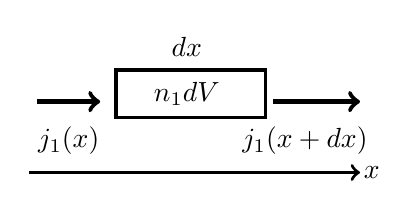
\begin{tikzpicture}
    \draw[black, very thick, ->] (-2,0) -- (2.2,0);
    \draw[black, line width=0.6mm, ->] (-2+0.1, 1-0.1) -- (-1-0.1,1-0.1);
    \draw[black, line width=0.6mm, ->] (-2+0.1+3, 1-0.1) -- (2.2,1-0.1);
    \draw[black, very thick] (-0.9,1-0.3) rectangle (1,2-0.7);
    \filldraw[black] (0,1)  node {$n_1 dV$};
    \filldraw[black] (-1.5, 0.4)  node {$\vc{j}_1(x)$};
    \filldraw[black] (1.5, 0.4)  node {$\vc{j}_1(x+dx)$};
    \filldraw[black] (0,1.6)  node {$dx$};
    \filldraw[black] (2.35,0)  node {$x$};
\end{tikzpicture}
    \caption{К выводу уравнения диффузии.}
\end{figure}
Таким образом приходим к уравнению баланса:
$
\ptdv{n_1}{t} + \ptdv{j_1}{x} = 0.
$\\
Воспользовавшись (\ref{fic}), получим
$$
\ptdv{(nc_1)}{t} = \ptdv{}{x} \lr{n D \ptdv{c_1}{x}}.
$$

При $u \neq 0$:
$$
j_1 = n \lr{-D \ptdv{c_1}{x} + c_1 u}
$$
Приходим у уравнению (\ref{konvec}).
\end{proof}

\noindent
\textbf{Уравнение непрерывности:}
\begin{equation}
    \ptdv{n}{t} + \nabla \cdot \vc{j} = 0, \hspace{1cm} \vc{j} = n \vc{u}
\end{equation}


\noindent
\textbf{Уравнение теплопроводности:}
\begin{equation}
    \begin{split}
        \boxed{\ptdv{T}{t} = \frac{\varkappa}{n C_P^{(1)}}\ptdv{^2T}{x^2} }
    \end{split} \hspace{1cm}
    \begin{split}
        \rho C_V^{(m)} \ptdv{T}{t} = \nabla \cdot (\varkappa \nabla(T))
    \end{split}
\end{equation}

\begin{proof}[$\triangle$]
\dots
\end{proof}
При постоянных характеричтиках вещества, придём к более простой форме:
\begin{equation}
    \ptdv{T}{t} = a \Delta T, \hspace{1cm} \Delta = \ptdv{^2}{x^2} + \ptdv{^2}{y^2} + \ptdv{^2}{z^2}.
\end{equation}

\noindent
\textbf{Уравнение\footnote{
    Где $q$ -- тепловой поток, $u$ -- энергия объёма $dV$.
} теплового баланса:}
\begin{equation}
    \ptdv{u}{t} + \ptdv{q}{x}=0
\end{equation}

\begin{table}
    \centering
    % \caption{А на самом деле..:}
        \begin{tabular}{rc|c|cc}
    \toprule
           & &формула&$\approx$&шары\\
    \midrule
            диффузия &$D_{12}$     
            & $\overline{v}_{\text{отн}}/((n_1+n_2)\sigma_{12})$
            &$1/3$ &$1/3$\\
            самодиффузия& $D_s$    
            & $\overline{v} \lambda$
            & \dots & $\sqrt{2}/3$\\
            вязкость &$\eta$       
            & $\rho \lambda \overline{v}$
            & $1/3$ & $1/(2 \sqrt{2})$\\
            теплопроводность &$\varkappa_1$
            & $n C_v^{(1)} \lambda \overline{v}  $
            & $1/3$ & $5/(4 \sqrt{2})$\\
            \hline
            \textcolor[gray]{0.5}{связь}
             &                  
            &\multicolumn{3}{c}{\com{
            $\frac{\eta}{\rho} = 
            \frac{3}{4} D_s =
            \frac{5}{2} \frac{\varkappa_1}{n C_V}$}
            }\\
    \bottomrule
        \end{tabular}
    \label{tab:}
\end{table}

\noindent
\textbf{Задача о расплывании облака:}
\begin{equation}
    n(x,t) = \frac{\const}{\sqrt{2Dt}} \exp \lr{-\frac{x^2}{4Dt}}
\end{equation}





